\chapter{Introducción}

En este capítulo no deben faltar los siguientes apartados:

\section{Motivación del proyecto}

En los últimos años el consumo de energía primaria en España ha aumentado significativamente de unos 88455 ktep($\sim1.03E12 \ kWh$) en 1990 a unos 126107 ktep($\sim 1.43E12 \ kWh$) en 2019, que equivale a un aumento del 42\% respecto a su valor en 1990, llegando a ser su valor máximo unos 146891 ktep($\sim 1.71E12 \ kWh$) en 2007.\\\\
De 2008 a 2014, como consecuencia de la crisis económica el consumo energético disminuyó hasta unos 117824 ktep ($\sim 1.37E12 \ kWh$) en 2014, recuperándose a partir del 2015, como se puede observar en la figura \ref{fig:demandaenergiaprimariaproporcion1990}. \\


\begin{figure}[H]
	\centering
	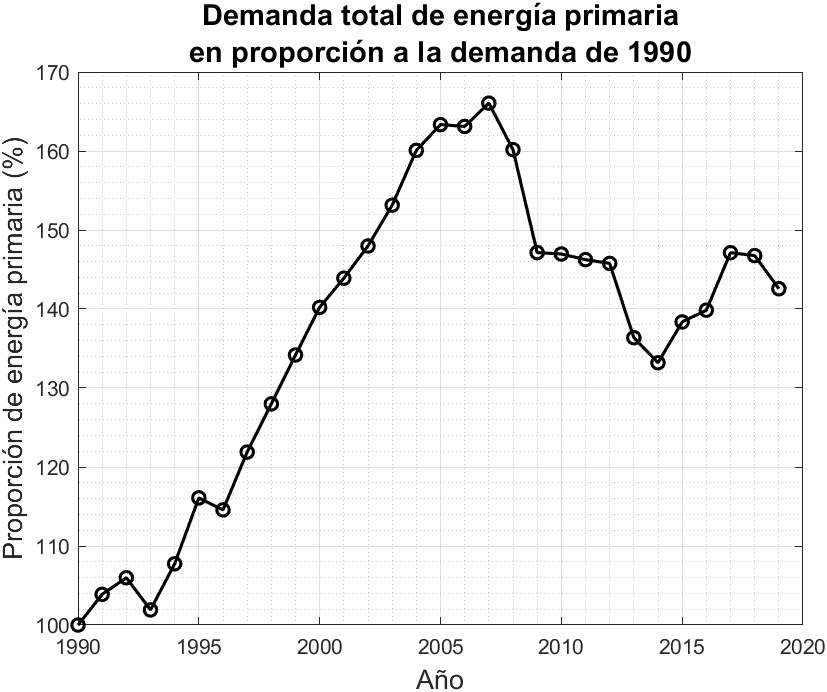
\includegraphics[width=10cm, height=7cm]{figuras/DemandaEnergiaPrimariaProporcion1990}
	\caption[Relación entre demanda total de energía primaria anual]{Representación gráfica de la relación entre la demanda total de energía primaria anual de 1990 hasta 2019 en España. \textit{Fuente obtención de datos: Ministerio para la transición ecológica y el reto demográfico de España.} }
	\label{fig:demandaenergiaprimariaproporcion1990}
\end{figure}
Dicha energía se puede dividir en diferentes categorías según el sector que la consume o la fuente de dicha energía. En el 2019, un 44.5\% de la energía primaria fue consumida de productos petrolíferos y apenas un 14.5\% de renovables (figura \ref{fig:fuentesenergiasprimarias}), y un 23.6\% de la energía final fue consumida por el sector de la industria (figura \ref{fig:consumoenergiafinalporsectores2019}), representando casi una cuarta parte del consumo total de la energía final en España. Desafortunadamente en todos los procesos energéticos, ya sean de producción, transporte o consumo, una parte de la energía siempre es desaprovechada en forma de calor (conocido como calor residual). En 2015, la industria en España consumió aproximadamente 220 TWh de energía, desperdiciándose unos 22 TWh según los cálculos de las estimaciones realizadas en \cite{wasteEnergyindustryEstimate}.

\begin{figure}[H]
	\centering
	\begin{subfigure}[b]{0.48\textwidth}
		\includegraphics[width=\textwidth]{figuras/FuentesEnergíasPrimarias}
		\caption{Consumo de energía por fuente}
		\label{fig:fuentesenergiasprimarias}
	\end{subfigure}
	\hfill
	\begin{subfigure}[b]{0.48\textwidth}
		\centering
		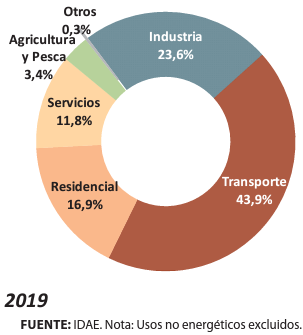
\includegraphics[width=\textwidth]{figuras/consumoEnergiaFinalPorSectores_2019}
		\caption{Consumo de energía por sectores.}
		\label{fig:consumoenergiafinalporsectores2019}
	\end{subfigure}
\caption[Desglose del consumo de energía primaria en España 20]{Desglose del consumo de energía primaria en España 2019 por fuente de energía(\subref{fig:fuentesenergiasprimarias}). Consumo de energía final por sectores en el año 2019 en España(\subref{fig:consumoenergiafinalporsectores2019}). \textit{Fuente:  Ministerio para la transición ecológica y el reto demográfico de España.} }
 \label{fig:consumosEnergiasCategorias}
\end{figure}

Para recuperar esta energía perdida se han desarrollado instalaciones de recuperación de calor residual, no solo para disminuir los costes sino también para disminuir las emisiones de contaminantes, cumpliendo así parte de los objetivos de desarrollo sostenible. El calor residual se puede aprovechar para obtener electricidad o para calentar un fluido para mejorar la eficiencia del mismo u otro proceso, disminuyendo el consumo de combustible u energía.\\

El aprovechamiento del calor residual para el calentamiento de otro fluido se utiliza en la industria, por ejemplo, un dispositivo llamado economizador que se usa en calderas para pre-calentar el fluido, mejorando el rendimiento térmico, o en el sector residencial que aprovecha el calor obtenido en el sistema de enfriamiento de algunos sistemas fotovoltaicos para obtener agua caliente.\\ 

La obtención de electricidad mediante el aprovechamiento del calor residual puede ser por vía de trabajo mecánico o por conversión directa. Por vía de trabajo mecánico se produce mediante ciclos termodinámicos, principalmente el ciclo de Rankine, el cual mediante un intercambiador de calor se genera vapor de agua que luego hace mover unas turbinas que están conectadas a un generador. La conversión directa se basa en la utilización de dispositivos termoeléctricos, termoiónicos, entre otros.\\

La conversión termo-eléctrica por vías mecánicas es la más conocida y es altamente utilizada, por ejemplo, las centrales nucleares, los sistemas de ciclos combinados, los sistemas de tratamientos de residuos que necesitan ser incinerados(figura \ref{fig:esquemaslomasvalorizacion}), entre otros. También se puede aprovechar el calor residual de la generación eléctrica, como es el caso de los cogeneradores.

%% IMAGENES DE SISTEMAS DE APROVECHAMIENTOS MECÁNICOS
\begin{figure}[H]
	\centering
	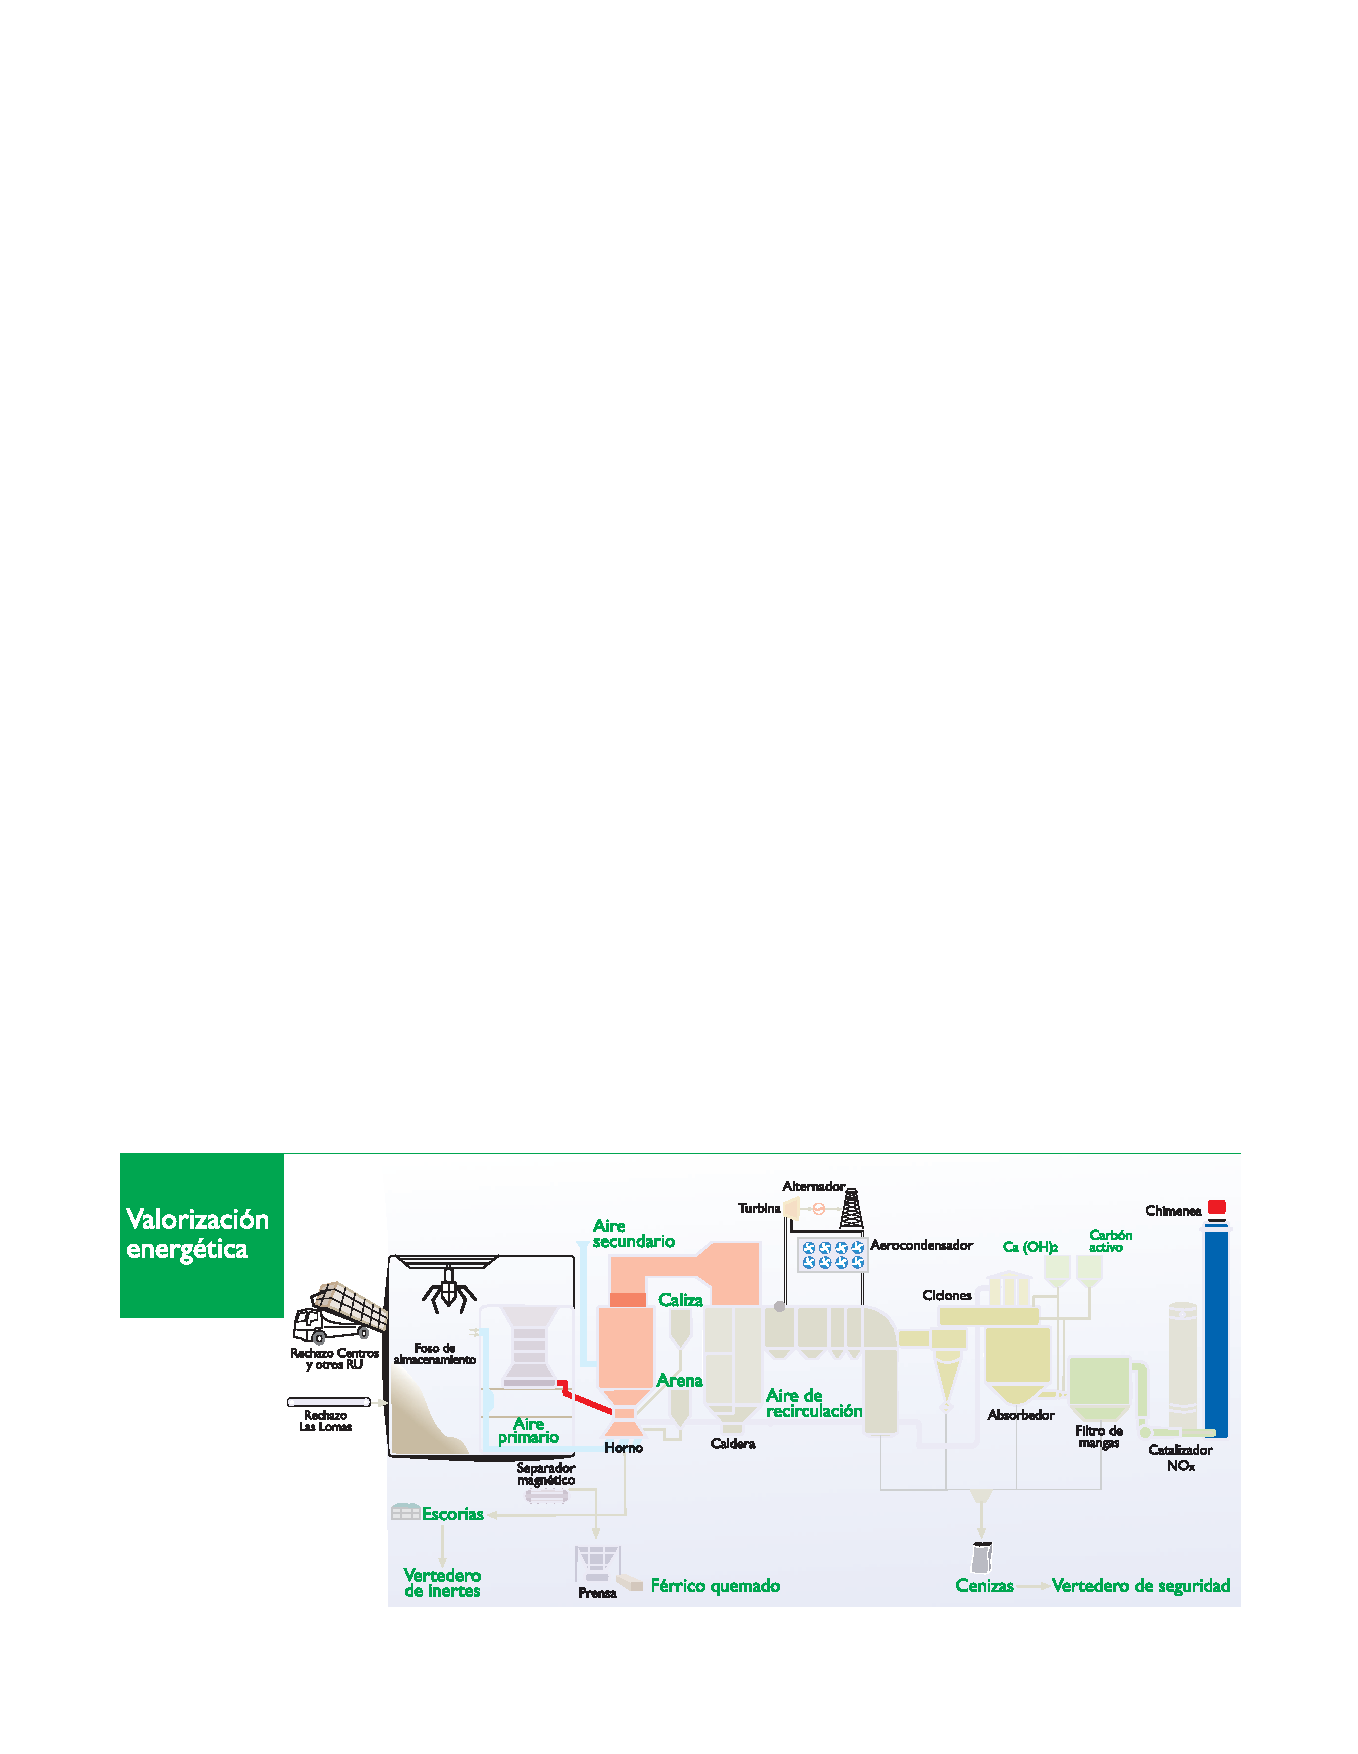
\includegraphics[height=5cm]{figuras/esquemasLomasValorizacion}
	\caption{Planta de valorización energética del Centro Las Lomas del Parque Tecnológico de Valdemingómez, donde se aprovecha los gases a alta temperatura para producir vapor de agua en la caldera para mover unas turbinas conectadas a generadores para producir electricidad. \textit{Fuente: Ayuntamiento de Madrid}}
	\label{fig:esquemaslomasvalorizacion}
\end{figure}

El problema principal con un sistema de este tipo son las partes móviles, las cuales tienen que estar en constante mantenimiento, para disminuir el mantenimiento se puede pasar a un sistema de recuperación de calor residual directo, ya sea con un dispositivo termoeléctrico, termoiónico o termofotovoltaico. Además de no presentar partes móviles o tener que tratar con fluidos, estos sistemas se pueden utilizar para varias aplicaciones, por ejemplo la espacial, donde la presión atmosférica es nula y la fuerza gravitacional total no es aproximadamente constante, o en la automoción donde se puede aprovechar las altas temperaturas de los motores para alimentar las luces o los circuitos electrónicos del vehículo.\\

% Termo Electrico
Los dispositivos termoeléctricos son dispositivos semiconductores, uno tipo n y otro tipo p, que están unidos en sus extremos que cuando se les aplica una diferencia de temperatura entre ambas uniones, se genera una diferencia de potencial, conocido como efecto Seebeck, que se utiliza para generar electricidad. Los materiales que se utilizan para estos dispositivos tienen unas conductividades térmicas bajas, para disminuir las pérdidas por conducción de calor, y aumentar el coeficiente Seebeck del generador termo-eléctrico (TEG) porque a mayor sea esta diferencia, mayor será la diferencia de potencial.\\

La eficiencia de los TEGs es alrededor del 5\%, aunque hasta el momento la eficiencia ha llegado como máximo hasta aproximadamente 15\%, lo cual sigue siendo demasiado baja. Aún con bajas eficiencias los TEG se utilizan para aplicaciones espaciales, recuperación de calor en el transporte,entre otros.\\


% Termoiónico
Otros sistemas de obtención de electricidad de una fuente de calor es la generación termoiónica (TIC), que mediante el emisión termoiónica se produce un flujo de electrones entre el emisor metálico a alta temperatura y un receptor a menor temperatura, separados por el vacío. Al aumentar la temperatura del emisor, los electrones libres se excitan hasta tal punto que la energía es lo suficientemente grande como para que se desprendan del material, la densidad de corriente está determinada por la ley de Richardson, donde $J=A\cdot T^2\cdot e^{\frac{-W}{k\cdot T}}$, siendo J la densidad de corriente, A la constante de Richardson, W la función de trabajo del metal, k la constante de Boltzman y T la temperatura en Kelvin.\\

% Termofotovoltaico
Un generador que se puede utilizar en conjunto con el TIC, es un generador termofotovoltaico (TPV) que transforman la radiación electromagnética producida por el emisor a alta temperatura para ser capturada por el receptor, que es una célula fotovoltaica. Los emisores de las TPV no tienen que estar a unas temperaturas tan altas como los TIC, ya que no necesita que se desprendan los electrones. Ambos dispositivos presentan el mismo problema de pérdidas de electrones o fotones por los bordes del convertidor y para disminuir esto se disminuye la separación entre el emisor y el receptor. Cuando las distancias se vuelven nanométricas aumenta la transferencias de fotones por la transferencia de radiación evanescente y/o electrones por la eliminación del efecto de carga de espacio, generando una mayor potencia eléctrica porque la potencia radiada aumenta por encima por la de un cuerpo negro según Planck.\\

La eficiencia de las TPVs han aumentado con el tiempo hasta llegar aproximadamente a un 40\% con una célula de dos uniones con materiales de bandas de energía entre 1 y 1.4 eV, utilizando un reflector trasero que devuelve la radiación de menor energía a la banda energética directa al emisor, pero solo llegando a obtener una densidad de potencia de 2.39 $W{cm}^{-2}$ \cite{ThermalConductivity_SiO2_2018}.\\

Los dispositivos que aprovechan los efectos de campo cercano presentan la dificultad de mantener la separación de manera constante por lo tanto se han fabricado y probado en varias ocasiones espaciadores de alturas desde un par de micras hasta unos pocos de cientos de nanómetros, con diferentes geometrías y materiales. Por ejemplo, en \cite{doi:MicroGapTPV} usan espaciadores de $1\mu m$ de $SiO_2$ y se observó que al disminuir la distancia de separación la corriente de cortocircuito aumenta.


\section{Objetivos}
El objetivo de este estudio es diseñar y simular pilares de dimensiones nanométricas para el aprovechamiento del efecto de campo cercano en un convertidor termo-fotovoltaico, así como determinar la viabilidad de este sistema. 
\begin{itemize}
	\item Modelar un nano-espaciador dentro de los rangos permitidos de los parámetros de los programas de simulación y modelado 3D.
	\item Modelar el emisor y la célula del sistema TPV para que los gradientes térmicos por conducción no lleguen a los bordes.
	\item Simular la transferencia de calor por conducción a través de un nano-espaciador de $SiO_2$ de un sistema TPV para diferentes alturas del nano-espaciador, diferentes materiales de emisor y diferentes resistencias de contacto entre emisor y el nano-espaciador.
	\item Simular la transferencia de calor radiada entre el emisor y la célula para diferentes materiales del emisor y para varias distancias de separación, teniendo en cuenta los efectos de campo cercano en la radiación.
	\item Determinar entre los casos estudiados cuales pueden dar lugar a sistemas de TPV de campo cercano viables.
\end{itemize}


\section{Estructura del documento}

A continuación y para facilitar la lectura del documento, se detalla el contenido de cada capítulo.

\begin{itemize}
\item En el \textbf{capítulo 1} se realiza una introducción del trabajo con la respectiva motivación y objetivos.
\item En el \textbf{capítulo 2} se desarrolla el estado de arte, definiendo los apartados más importantes y resaltando las investigaciones con mayor relevancia.
\item En el \textbf{capítulo 3} se exponen las herramientas y materiales utilizados, así como los criterios de selección.
\item En el \textbf{capítulo 4} se mencionan los métodos seguidos y los cálculos realizados para el desarrollo del trabajo.
\item En el \textbf{capítulo 5} se exponen los resultados obtenidos de las simulaciones.
\item En el \textbf{capítulo 6} se desarrolla la conclusión y se realiza planteamientos para futuros trabajos.
\end{itemize}
